%=====================================================================
\section{Methods}
\label{sec:methods}
Every analysis follows the same template: hypothesis from the literature $\to$ metric
$\to$ randomized reference model. \Cref{tab:hypotheses} lists the seven hypotheses,
the methods (M1--M4) that test them and the datasets where each method is meaningful
(19 method--dataset pairs). The empty cells are deliberate: CIT is a year-resolution
DAG without fine-grained events (no M2a, M2b, M3) and without community
reorganisation (no M4), while PS and CM have no growth process (no M2c).

\begin{table*}[t]
\centering
\small
\setlength{\tabcolsep}{4pt}
\begin{tabular}{@{}cl p{6.2cm} l l l ccc@{}}
\toprule
Part & ID & Hypothesis & Source & Method & Null & PS & CM & CIT \\
\midrule
I   & H1 & Aggregation and window choice change structural conclusions
           & \citep{krings2012effects,ribeiro2013quantifying} & M1 & -- & \checkmark & \checkmark & \checkmark \\
\midrule
II  & H2 & Activity is bursty and has memory
           & \citep{goh2008burstiness} & M2a & P1 & \checkmark & \checkmark & \\
    & H3 & Ties are repeated and persistent; the network turns over
           & \citep{saramaki2014persistence} & M2b & P1 & \checkmark & \checkmark & \\
\midrule
III & H4 & Growth follows preferential attachment with ageing; networks densify
           & \citep{jeong2003measuring,wang2013quantifying,leskovec2005graphs} & M2c-1--4 & P3 & & & \checkmark \\
    & H5 & Communities reorganise over time; the static partition hides this
           & \citep{greene2010tracking,mucha2010community} & M4 & P1 & \checkmark & \checkmark & \\
\midrule
IV  & H6 & Time ordering restricts reachability and changes centrality rankings
           & \citep{holme2005network,pan2011path,kim2012temporal} & M3a, M3b & P1, P2 & \checkmark & \checkmark & \\
    & H7 & Burstiness and temporal correlations slow down spreading
           & \citep{karsai2011small} & M3c & P1, P2 & \checkmark & \checkmark & \\
\bottomrule
\end{tabular}
\caption{Hypotheses tested in this work, with methods, null models
(\cref{sec:null}) and applicable datasets.}
\label{tab:hypotheses}
\end{table*}

\subsection{Notation}
\label{sec:notation}
Let $\mathcal{E}=\{(u,v,t)\}$ be the event sequence. The static aggregate $G$
contains a link $(u,v)$ if at least one event occurs between $u$ and $v$. A
snapshot $G_{\Delta t}(k)$ contains the events in $[k\Delta t,(k+1)\Delta t)$, and the
cumulative network $G(\le t)$ contains all events up to $t$.

\subsection{Aggregation and time windows (M1)}
\label{sec:m-aggregation}
For each window length $\Delta t$ on a grid (PS: 5\,min to 1\,day; CM: 1\,h to 1\,month)
we compute density, mean degree, clustering coefficient and giant-component size of the
snapshots and of the aggregate. For CIT, yearly and cumulative networks are compared.
\emph{Window sensitivity} is the relative change of a metric across the grid.
Rankings are handled separately in M3b. \Cref{fig:aggschem} shows why aggregation can
mislead: a path present in the static graph may not be traversable in time.

\begin{figure*}[t]
\centering
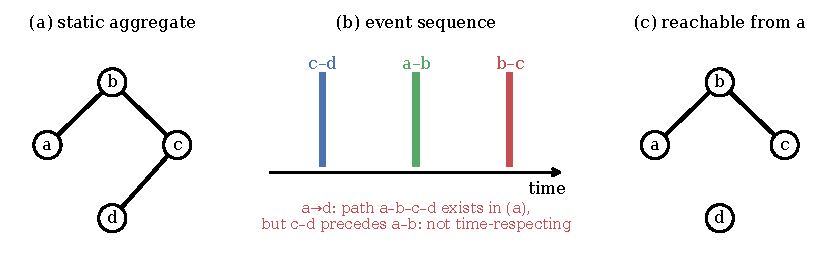
\includegraphics[width=0.7\linewidth]{fig_aggregation_schematic.pdf}
\caption{Aggregation adds paths that do not exist in time. In (a) $a$ appears to
reach $d$; in (b) the link $c$--$d$ is active before $a$--$b$, so in (c) only $b$ and
$c$ are reachable from $a$.}
\label{fig:aggschem}
\end{figure*}

\subsection{Activity patterns (M2a, M2b)}
\label{sec:m-activity}
\textbf{M2a} measures the inter-event time distribution of each node pair and of each
node, fitted with a heavy-tailed model, together with burstiness
$B=(\sigma-\mu)/(\sigma+\mu)$ and memory $M$, the correlation of consecutive
intervals \citep{goh2008burstiness}. \textbf{M2b} measures the edge repetition rate,
tie lifetime and the Jaccard similarity of consecutive snapshots, which quantifies
the turnover of nodes and links.

\subsection{Structural evolution (M2c, M4)}
\label{sec:m-evolution}
% Owner: B (expanded M2c-1 through M2c-4 and P3).
% Owner: B. Measured-result-independent methods, PLAN v3.1.
\paragraph{Citation data and time resolution.}
We stream AMiner DBLP-Citation V14 \citep{tang2008arnetminer} and retain an induced subgraph of database
venues selected by a fixed whitelist (SIGMOD, VLDB/PVLDB, ICDE, PODS, EDBT,
ICDT, TODS, VLDB Journal, Data \& Knowledge Engineering, and Information Systems).
All selected papers published in 1960--2020 are retained, including isolates.
A distinct citation $u\to v$ occurs in the publication year of $u$.
The primary analysis requires $y_v<y_u$; same-year citations are saved for
structural sensitivity analysis because their order cannot be resolved.
We exclude self-citations to the same paper, duplicate edges and future references.
Author self-citations are not removed. Counts refer to citations within the
selected venues, rather than global citation impact. The primary analysis years
are 1990--2020, initialized using the available earlier history.

\paragraph{M1: annual and cumulative citation structure.}
Annual and cumulative networks use the same node denominator: all selected
papers already published by year $t$. Directed density is $E/[N(N-1)]$ and
mean total degree is $2E/N$. Clustering, component counts and largest-component
fractions use the weak undirected projection, including isolates.
Trailing windows of 1, 2, 5 and 10 years provide a window-sensitivity check;
sensitivity is $(\max-\min)/\mathrm{mean}$ over the grid at each endpoint,
then averaged over endpoints.

\paragraph{M2c-1: preferential attachment.}
Following the degree-class approach of \citet{jeong2003measuring}, we freeze
in-degree at the start of each citing year and count eligible nodes $n_{tk}$ and
new citations $h_{tk}$ in each prior-degree class $k$.
We estimate $\alpha$ by conditional likelihood with probabilities proportional
to $n_{tk}(k+1)^\alpha$, conditioning on the total number of citations in each year.
The offset admits citations to previously uncited papers; offsets 0.5 and 2
provide sensitivity checks. Confidence intervals use 400 resamples of citing-year
blocks. These are descriptive uncertainty intervals; neither positive $\alpha$
nor its departure from an age-only null identifies a causal mechanism.

\paragraph{M2c-2: ageing.}
For ages 1--60, the target probability in citing year $t$ is proportional to
$n_{ta}f(a)$, where $n_{ta}$ counts available papers of age $a$.
A conditional target likelihood compares discrete-grid lognormal, exponential,
power-law and uniform kernels using AIC on identical observations and support.
We repeat the comparison by publication cohort (1970--1989, 1990--1999,
2000--2009), accounting for each cohort's actual exposure.
This estimates marginal ageing; degree, fitness and venue coverage can also
influence this curve.

\paragraph{M2c-3: densification and diameter.}
We fit $\log E(t)=a\log N(t)+b$ over 1990--2020 and repeat over split periods and
an earlier observation cutoff. Year-resampling intervals are descriptive because
cumulative observations are dependent.
Effective diameter is the 90th percentile of weak shortest-path distances
within the largest connected component, using 128 uniformly sampled source nodes
per year. Sensitivity checks use 64 and 256 sources. We save the component size
and number of sources with every estimate \citep{leskovec2005graphs}.

\paragraph{M2c-4: citation dynamics and prediction.}
We fit the Wang--Song--Barab\'asi curve \citep{wang2013quantifying},
\begin{equation}
 c(t)=m\left[\exp\!\left\{\lambda\Phi\left(\frac{\log t-\mu}{\sigma}\right)\right\}-1\right],
\end{equation}
where $m$ is fixed to the mean observed within-subgraph reference count of papers
published through 1989. Bounded multistart least squares minimizes squared
$\log(1+c)$ errors; parameter bounds and boundary flags are preserved.
For descriptive full-history fits we randomly select at most 500 papers born in
1990--2005 with at least 10 citations by age 15 and fit years 1--15. The resulting
collapse is in-sample evidence only.
For prediction, selection uses only the first five years: at least five observed
citations by age five, followed by a fixed random sample of at most 500 papers.
Using only years 1--5, we compare WSB against no-ageing PA,
$c(t)=m[\exp(rt)-1]$, and linear extrapolation, $c(5)t/5$.
All models predict the same papers at age 15 and at the observed endpoint in 2020;
these are censored observed totals, not unobserved lifetime citations.
We report MAE, median absolute error, RMSLE, paired bootstrap differences
(1000 resamples) and an interior-fit sensitivity check. Boundary fits remain in
the primary evaluation so that difficult cases are not silently discarded.

\paragraph{P3: citation-target randomization.}
Twenty realizations per model preserve each paper's publication year and exact
number of distinct observed references, with no replacement and strictly older
targets. P3a selects eligible targets uniformly. P3b weights targets by a nonparametric age kernel fitted by conditional
target likelihood, accounting for each citing year's available age distribution,
and removes degree preference.
Its age weights are calibrated from the data, so agreement on ageing is not an
independent confirmation. We report null means and sample standard deviations;
empirical tail probabilities have minimum resolution $1/21$.
Both models fix $N(t)$ and $E(t)$ and hence exactly preserve the densification
exponent. They can test diameter and target preference, but cannot supply a
significance test for densification itself.

\paragraph{Reproducibility.}
All significant CPU workloads run on Vanda compute nodes through PBS without GPU
allocation. Fixed seeds, input/source checksums, environment lock file, filtering
counts, individual forecasts and every randomized edge list are saved.
Robustness checks cover time splits, cutoff 2015, degree offsets, same-year edges,
core database venues, diameter sampling, and 10 versus 20 null realizations.


% Owner: E
% Owner: E. M4 (H5), input from methods.tex.
\textbf{M4} cuts the event sequence into consecutive windows of width $\Delta t$ and
aggregates each into a weighted undirected snapshot (weight = number of events). Windows
with very few events are dropped (fewer than 100 for PS, which removes nights; fewer
than 50 for CM), and only nodes active in a window belong to its snapshot. The main
settings are $\Delta t=15$\,min for PS and 7\,days for CM. Every snapshot and the
static aggregate are partitioned with Leiden \citep{traag2019louvain} maximising
modularity with resolution $\gamma$ \citep{reichardt2006statistical}. A multislice
partition \citep{mucha2010community} with interslice coupling $\omega=1$ gives labels
that are consistent across windows; we use it only for tracking, because the coupling
itself pulls consecutive partitions together.

Partitions are compared with NMI \citep{danon2005comparing}, always on the nodes the two
partitions share. For each window we record the NMI with the previous window (only for
back-to-back windows, not across a night), with the static partition, and for PS with
the classes (teachers excluded). As a noise floor, every window is partitioned a second
time with another random seed. All measures are recomputed on 20 P1 samples: P1 keeps
the static graph, and hence the static partition, and the number of events per window,
so H5 predicts that real snapshots agree less with each other and with the static
partition than P1 snapshots do. We repeat the analysis for $\gamma\in\{0.5,1,2\}$ and
$\Delta t\in\{5,15,60\}$\,min (PS) or $\{1,7,30\}$\,days (CM).


\subsection{Paths, centrality and spreading (M3)}
\label{sec:m-function}
\textbf{M3a} computes earliest-arrival time-respecting paths and the temporal reachability
ratio $R$ (fraction of node pairs connected by a time-respecting path, relative to the
static aggregate). \textbf{M3c} runs an event-driven SIR process on the event sequence with
at least 100 random seeds; SI with certain transmission is equivalent to M3a, so only SIR
is run.

% Owner: E
% Owner: E. M3b (H6), input from methods.tex.
\textbf{M3b} compares static and temporal closeness. Static closeness is harmonic
closeness \citep{marchiori2000harmony}, $C^{\mathrm{s}}(i)=\sum_{j\neq i}1/d(i,j)$, on
the aggregate (outgoing distances for CM), with hop distance (unweighted) or distance
$1/w_{ij}$ (weighted). Temporal closeness \citep{pan2011path,kim2012temporal} uses the
same time-respecting paths as M3a: from a start time $t_0$, an event $(u,v,t)$ can be
used only if $u$ was reached strictly before $t$, and $v$ is then reached at $t$, so no
path takes two hops within one timestamp. With $a_{t_0}(i\to j)$ the earliest arrival
time,
\begin{equation}
  C^{\mathrm{t}}(i)=\frac{1}{|\mathcal{T}|}\sum_{t_0\in\mathcal{T}}\frac{1}{N-1}
  \sum_{j\neq i}\frac{1}{a_{t_0}(i\to j)-t_0},
\end{equation}
where unreachable nodes contribute zero. $\mathcal{T}$ holds every full hour from
09:00 to 16:00 on both PS days (16 start times) and 20 evenly spaced times over the
first 90\% of the CM period. Agreement is measured by Kendall's $\tau_b$ and the overlap
of the top 10\% nodes. P1 leaves the static graph and so $C^{\mathrm{s}}$ unchanged;
recomputing $C^{\mathrm{t}}$ on 20 P1 samples therefore isolates the effect of timing.


\subsection{Randomized reference models}
\label{sec:null}
No single temporal counterpart of the configuration model exists, so one switches off
selected correlations with different models and compares the outcomes
\citep{holme2012temporal,gauvin2022randomized}. For PS and CM we use two complementary models, which
correspond to \emph{randomly permuted times} (RP) and \emph{randomized edges} (RE) in the
naming of \citet{holme2012temporal}. \textbf{P1} (RP) permutes timestamps among events:
it keeps the static graph and the number of contacts of every pair, and destroys
burstiness and temporal correlations. \textbf{P2} (RE) rewires the static graph in a
degree-preserving way while each pair's contact sequence moves with its link: it
destroys the wiring diagram but keeps per-link burstiness and the overall event rate
(\cref{fig:nullmodels}). Comparing the two separates the effect of time from that of
structure. Combined models (RE+RP) and fully random times (RT) are possible extensions. Each is run with at least
20 realisations and reported as mean $\pm$ standard deviation.

\begin{figure*}[t]
\centering
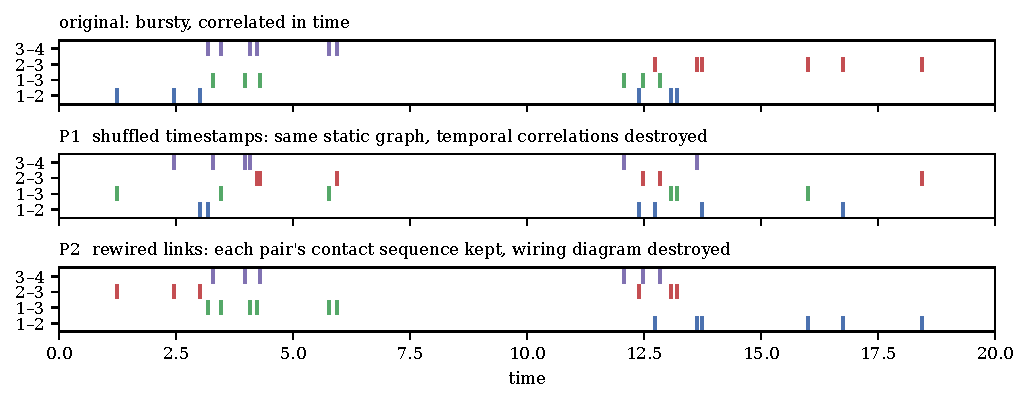
\includegraphics[width=\linewidth]{fig_nullmodels.pdf}
\caption{Toy illustration of the randomized reference models. Rows are node pairs,
ticks are events. P1 permutes the timestamps, P2 permutes which pair each event
belongs to.}
\label{fig:nullmodels}
\end{figure*}

\subsection{Measuring the effect of time}
\label{sec:time-effect}
Raw metrics cannot be compared across a contact network, a message network and a
citation network, so we define one normalised measure per hypothesis:
H1 window sensitivity (relative change of a metric over the $\Delta t$ grid);
H2 $B_{\mathrm{real}}-B_{\mathrm{null}}$;
H3 mean consecutive-snapshot Jaccard similarity;
H4 exponents $\alpha$ and $a$;
H5 mean consecutive-snapshot NMI and dynamic-vs-static NMI;
H6 reachability ratio $R$ and Kendall $\tau$(static, temporal);
H7 slowdown $T_{\mathrm{real}}/T_{\mathrm{null}}$, where $T$ is the time to the epidemic peak.

\subsection{Implementation}
All code is in Python. We use NetworkX for static graph analysis and leidenalg
\citep{traag2019louvain} for per-snapshot and multislice partitions; time-respecting
paths are computed by our own earliest-arrival code. Null models, the attachment-kernel
% E: Raphtory and tnetwork were planned but not used (M3b, M4); D to confirm for M3a.
estimator and the SIR process are custom code, unit-tested on hand-built examples
whose answers are known (reachability, SIR, preserved quantities of P1 and P2). Random
seeds are fixed and every figure is generated by one script.
